\documentclass[a4paper,14pt]{report}
\usepackage[utf8]{inputenc}
\usepackage[T1]{fontenc}
\usepackage{titlesec}
\usepackage{float}
\usepackage{graphicx}
\graphicspath{ {./wykresy/} }

\renewcommand{\contentsname}{Spis treści}

\titleformat{\chapter}[display]
  {\normalfont\bfseries}{}{0pt}{\Huge}

\usepackage{pgfplots}
 
\pgfplotsset{compat = newest}

\title{Obliczenia naukowe Lista 2}
\author{Radosław Wojtczak}
\date{Numer indeksu: 254607}
\begin{document}
\maketitle
\tableofcontents


\chapter{Zadanie 1.}
  \section{Krótki opis problemu}
    Problematyką tego zadania było sprawdzenie, jak zmiana danych wejściowych wpływa na otrzymane wyniki. Porównania dokonujemy z zadaniem 5 z listy 1.
  \section{Rozwiązanie}
    Rozwiązanie wygląda identycznie do rozwiązania z zadania 5 listy 1 z odpowiednio zmienionymi wartościami $x_{4}$ i $x_{5}$ 
  \section{Wyniki oraz ich interpretacje}
    Poniższe tabele prezentują porównanie otrzymanych wyników z wynikami z poprzedniej listy. \\
    Dokładna wartość: \textbf{-1.00657107000000e-11}
    \begin{table}[h!]
    \centering
    \begin{tabular}{|c | c | c |} 
     \hline
     Algorytm & Lista1Zad5 & Lista2Zad1 \\ [0.5ex] 
     \hline\hline
     1. & -0.4999443 & -0.4999443  \\ 
     2. & -0.4543457 & -0.4543457 \\
     3. & -0.5 & -0.5 \\
     3. & -0.5 & -0.5 \\
     \hline
    \end{tabular}
    \caption{Otrzymane wyniki dla typu danych Float32}
    \label{Zad1Float32}
    \end{table}

    \begin{table}[h!]
    \centering
    \begin{tabular}{|c | c | c |} 
     \hline
     Algorytm & Lista1Zad5 & Lista2Zad1 \\ [0.5ex] 
     \hline\hline
     1.& 1.0251881368296672e-10 & -0.004296342739891585 \\ 
     2. & -1.5643308870494366e-10 & -0.004296342998713953 \\
     3. & 0.0 & -0.004296342842280865 \\
     3. & 0.0 & -0.004296342842280865 \\
     \hline
    \end{tabular}
    \caption{Otrzymane wyniki dla typu danych Float64}
    \label{Zad1Float64}
    \end{table}
    \textbf{Interpretacja :} Automatycznie zauważamy, iż mimo braku jakichkolwiek zmian w wykorzystanych algorytmach wartości w tabeli \ref{Zad1Float32} są identyczne, natomiast wartości w tabeli \ref{Zad1Float64} różnią się. Zmiany te wynikają z faktu, iż modyfikacja danych wejściowych o najmniejszą cyfrę znacząca (która w tym przypadku jest rzędu $10^{-10} $) jest inaczej zapamiętywana przez zmienne w standardzie Float32 jak i Float64, ze względu na różnicę liczby bitów wykorzystanych na zapamiętanie mantysy. Float32 nie widzi różnicy, gdyż wszystkie zmiany zachodzą w cyfrach, które wykraczają poza zakres mantysy, natomiast Float64 obejmuje swoim obszarem mantysy zmiany, co widzimy w otrzymanych powyżej wynikach.
  \section{Wnioski}
    Niewielkie zmiany w danych wejściowych prowadzą do znacznych zmian w wynikach- przykład źle uwarunkowanego zadania (jakim faktycznie jest mnożenie skalarne wektorów bliskich prostopadłości).

\chapter{Zadanie 2.}
  \section{Krótki opis problemu}
    Problematyką tego zadania było graficzne przedstawienie funkcji
    \begin{equation}
      f(x)=e^{x}*ln(1+e^{-x})
    \end{equation}
    w co najmniej dwóch programach do wizualizacji danych oraz porównanie otrzymanych wyników z wyznaczoną granicą
    \begin{equation}
      \lim_{x\to\infty} f(x)
    \end{equation}
  \section{Rozwiązanie}
    W swoim rozwiązaniu użyłem następujących programów do wizualizacji danych:
    \begin{itemize}
      \item Serwis internetowy WolframAlpha
      \item Program w pythonie z użyciem biblioteki \textit{matplotlib}
    \end{itemize}
  \section{Wyniki oraz ich interpretacje}
    Najpierw obliczamy granicę funkcji $f(x)$, która wynosi
    \begin{equation}
      f(x)=e^{x}*ln(1+e^{-x})=1
    \end{equation}
    Następnie analizujemy otrzymane wykresy: \\
    \begin{figure}[H]
      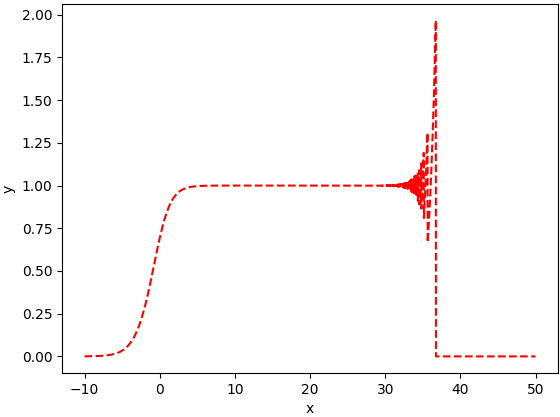
\includegraphics[scale=0.8]{wykresPython}
      \centering
      \caption{Wykres wykonany przez program w Pythonie}
    \end{figure}
    \begin{figure}[H]
      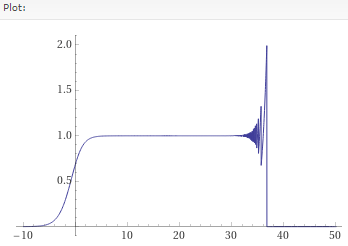
\includegraphics[scale=1.5]{wykresWolfram}
      \centering
      \caption{Wykres wykonany przez stronę WolframAlpha}
    \end{figure}
    \textbf{Interpetacja: } Otrzymane wykresy są niezgodne z naszymi oczekiwaniami. Do osiągnięcia wartości $x=30$ wszystko przedstawia się tak, jakbyśmy to zakładali, jednakże od tego momentu dochodzi do "odbiegania" od docelowej wartości 1. Zauważamy, że otrzymane wyniki stają się coraz bardziej oddalone od prostej $y=1$ aż do momentu, gdy od $x=37$ wartości zerują się. \\
    Sprawdźmy wartości $e^{-x}$ dla $x=36$, $x=37$ i porównajmy je z epsilonem maszynowym dla Float64 obliczonym w pierwszym zadaniu listy 1.
    \begin{table}[H]
    \centering
    \begin{tabular}{|c | c |} 
     \hline
     Funkcja & Wartość \\ [0.5ex] 
     \hline\hline
     $e^{-36} $ & 2.3195228302435696e-16\\
     \textit{macheps} & 2.220446049250313e-16 \\ 
     $e^{-37} $ & 8.533047625744066e-17\\
     \hline
    \end{tabular}
    \caption{Porównanie wartości $e^{-x}$ z epsilonem maszynowym}
    \label{Zad2Tabela}
    \end{table}
    Zauważamy, że wartość epsilona maszynowego dla standardu Float64 znajduje się między wartościami funkcji $e^{-x} $ dla wybranych powyżej wartości \textit{x}. Z tego powodu dochodzi do wyzerowania składnika $e^{-x}$ co prowadzi do tego, że otrzymujemy $ln(1)=0$, a wiadomo, że cokolwiek pomnożone razy 0 w wyniku daje 0.
  \section{Wnioski}
    Przy wykonywaniu obliczeń, w których operujemy na dużych, jak i małych wartościach, należy pamiętać o ograniczeniach sprzętowych. W powyższej sytuacji dodawanie liczb znacznie różniących się od siebie oraz ograniczenie reprezentacji liczb ze względu na limitowaną pamięć doprowadziły do sytuacji, że od pewnego x wyrażenie $e^{-x}$ było nierozróznialne od zera.
\chapter{Zadanie 3.}
  \section{Krótki opis problemu}
    Problematyką zadania było rozwiązanie układu równań liniowych
    \begin{equation}
      \textbf{Ax=b}
    \end{equation}
    gdzie \textbf{b} jest wektorem prawych stron zadany powyższym wzorem, $ \textbf{x}=(1,...,1)^{T} $ oraz A jest wygenerowaną macierzą w jeden z poniższych sposobów:
    \begin{itemize}
      \item \textbf{$A=H_{n}$} , gdzie \textbf{$H_{n}$} jest macierzą Hilberta
      \item \textbf{$A=R_{n}$} , gdzie \textbf{$R_{n}$} jest losową macierzą stopnia \textbf{n} z wskaźnikiem uwarunkowania \textbf{c}
    \end{itemize}
    przy pomocy dwóch algorytmów:
    \begin{itemize}
      \item Eliminacji Gaussa
      \item Inwersji ($x=A^{-1}b$ ($x=inv(A)*b)$)
    \end{itemize}

  \section{Rozwiązanie}
    W pliku zad3.jl znajdują się dwie funkcje Pana Profesora Zielińskiego (\textit{matcond() i hilb()}), które odpowiedzialne są za generowanie wyżej wspomnianych macierzy. \\
    Dodatkowo funkcje \textit{hilberts() i randoms()} odpowiadają za przeprowadzenie testów dla odpowiednich wartości wejściowych (Dla macierzy Hilberta z rosnącym stopniem $n>1$, dla macierzy losowej z $n=5,10,20$ oraz z $c=1,10,10^{3},10^{7},10^{12},10^{16}$.
  \section{Wyniki oraz ich interpretacje}
    Wyniki otrzymane w ramach uruchomienia programu zad3.jl przedstawione są w poniższych tabelach: 
    \begin{table}[H]
    \centering
    \begin{tabular}{|c | c | c | c | c |} 
     \hline
     Rozmiar & Rząd & cond & norma(inverse) & norma(gauss) \\ [0.5ex] 
     \hline\hline
     1 & 1 & 1.000000e+00 & 0.000000e+00 & 0.000000e+00 \\
     2 & 2 & 1.928147e+01 & 5.661049e-16 & 1.404333e-15 \\
     3 & 3 & 5.240568e+02 & 8.022594e-15 & 0.000000e+00 \\
     4 & 4 & 1.551374e+04 & 4.637278e-13 & 7.542471e-13 \\
     5 & 5 & 4.766073e+05 & 1.769706e-13 & 7.456028e-12 \\
     6 & 6 & 1.495106e+07 & 3.496491e-10 & 3.533152e-10 \\
     7 & 7 & 4.753674e+08 & 1.317505e-08 & 6.190844e-09 \\
     8 & 8 & 1.525758e+10 & 2.487433e-07 & 3.775275e-07 \\
     9 & 9 & 4.931541e+11 & 9.643625e-06 & 1.165949e-05 \\
     10 & 10 & 1.602486e+13 & 2.203529e-04 & 3.357159e-04 \\
     11 & 10 & 5.221035e+14 & 6.022513e-03 & 1.113777e-02 \\
     12 & 11 & 1.725543e+16 & 1.950924e-01 & 1.621862e-01 \\
     13 & 11 & 7.126492e+17 & 7.894192e+00 & 3.058359e+00 \\
     14 & 11 & 6.101308e+17 & 8.270688e-01 & 4.176748e+00 \\
     15 & 12 & 4.223311e+17 & 3.103493e+00 & 5.603159e+00 \\
     16 & 12 & 3.535828e+17 & 9.083115e+00 & 3.927234e+01 \\
     17 & 12 & 3.118281e+17 & 4.243292e+00 & 7.494042e+00 \\
     18 & 12 & 1.563917e+18 & 4.786030e+00 & 5.759995e+00 \\
     19 & 13 & 1.327444e+18 & 6.114994e+00 & 1.230921e+01 \\
     20 & 13 & 2.277764e+18 & 1.912224e+01 & 1.703082e+01 \\
     \hline
    \end{tabular}
    \caption{Wyniki dla macierzy Hilberta}
    \label{Zad3Hilbert}
    \end{table}
    \begin{table}[H]
    \centering
    \begin{tabular}{|c | c | c | c | c |} 
     \hline
     Rozmiar & Rząd & cond & norma(inverse) & norma(gauss) \\ [0.5ex] 
     \hline\hline
     5 & 5 & 1.000000e+00 & 3.020133e-16 & 2.328823e-16 \\
     5 & 5 & 1.000000e+01 & 3.020133e-16 & 2.432377e-16 \\
     5 & 5 & 1.000000e+03 & 2.655044e-14 & 3.370400e-14 \\
     5 & 5 & 1.000000e+07 & 3.129528e-10 & 2.968020e-10 \\
     5 & 5 & 9.999866e+11 & 3.482249e-06 & 8.357583e-06 \\
     5 & 4 & 1.175332e+16 & 7.238830e-02 & 5.226790e-01 \\
     10 & 10 & 1.000000e+00 & 1.313634e-16 & 2.135557e-16 \\
     10 & 10 & 1.000000e+01 & 2.328823e-16 & 3.385725e-16 \\
     10 & 10 & 1.000000e+03 & 9.466759e-15 & 9.733560e-15 \\
     10 & 10 & 1.000000e+07 & 2.222069e-10 & 1.994064e-10 \\
     10 & 10 & 9.999966e+11 & 1.122532e-05 & 1.249277e-05 \\
     10 & 9 & 6.130269e+15 & 6.814602e-01 & 6.018465e-01 \\
     20 & 20 & 1.000000e+00 & 5.248667e-16 & 6.240994e-16 \\
     20 & 20 & 1.000000e+01 & 5.932166e-16 & 3.821813e-16 \\
     20 & 20 & 1.000000e+03 & 5.626268e-15 & 6.784180e-15 \\
     20 & 20 & 1.000000e+07 & 1.845557e-10 & 2.512406e-10 \\
     20 & 20 & 9.999484e+11 & 1.821880e-05 & 2.024762e-05 \\
     20 & 19 & 9.050241e+15 & 1.398000e-01 & 1.037769e-01 \\
     \hline
    \end{tabular}
    \caption{Wyniki dla macierzy wygenerowanej losowo}
    \label{Zad3Random}
    \end{table}
    \textbf{Interpretacja: } Zauważamy, iż macierz Hilberta jest macierzą źle uwarunkowaną. Otrzymane wartości pokrywają się z wartościami podanymi przez wykładowcę na wykładzie ($ H_{6} ~ 1.5*10^{7} $ (u nas 1.495106e+07) oraz $ H_{10} ~ 1.6*10^{13} $ (u nas 1.602486e+13)). Zauważamy również, że wskaźnik cond(H) ciągle wzrasta.
  \section{Wnioski}
    W zależności od wartości wskaźnika uwarunkowania zadania otrzymujemy różne błędy (przedstawione w powyższej tabeli w kolumnach \textit{norm(inverse)} oraz \textit{norm(gauss)}). Mimo tak skutecznych i stabilnych metod jak metoda Gaussa czy zastosowanie inwersji praca na źle uwarunkowanych macierzach skutkuje dużymi błędami.

\chapter{Zadanie 4.}
  \section{Krótki opis problemu}
    Głównym celem tego zadania było odtworzenie doświadczenia Wilkinsona z wykorzystaniem "złośliwego wielomianu". Korzystając z pakiety Polynomials należało obliczyć 20 zer wyżej wspomnianego wielomianiu. Dodatkowo należało zaimplementować funkcję liczącą ten sam wielomian przy pomocy wartości iloczynowej. \\
    Następym krokiem w zadaniu było sprawdzić obliczone pierwiastki $1 \leq k \leq 20 $ obliczającac:
    \begin{itemize}
      \item $ |P(z_{k})| $
      \item $ |p(z_{k})|$
      \item $ |z_{k}-k|$
    \end{itemize}
    W drugim podpunkcie zadania należało zaburzyć wielomian poprzez podmianę jednego ze współczynników z wartości $-210$ na wartość $-210-2^{-23}$ oraz wykonać wszystkie powyższe operacje.
  \section{Rozwiązanie}
    Rozwiązanie zadania znajduje się w pliku zad4.jl. Rozwiązanie odbywa się w następujących krokach:
    \begin{itemize}
      \item Zaimportowanie odpowiednich współczynników do tablicy odpowiednio \textit{coefficientsA} dla podpunktu a oraz \textit{coefficientsB} dla podpunktu B.
      \item Utworzenie wielomianu ze współczynników podanych w powyższych tablicach przy pomocy metody \textit{Polynomial()}.
      \item Znalezienie miejsc zerowych przy pomocy funkcji \textit{roots()}.
      \item Obliczenie w pętli odpowiednich wartości podanych w krótkim opisie problemu.
    \end{itemize}
  \section{Wyniki oraz ich interpretacje}
    Otrzymane wyniki przedstawione są w poniższych tabelach:

    \begin{table}[H]
    \centering
    \begin{tabular}{|c | c | c | c | c |} 
     \hline
     k & |$P(z_{k})$| & |$p(z_{k})$| & |$z_{k}-k$| \\ [0.5ex] 
     \hline\hline
     1 & 3.635200e+04 & 3.662643e+04 & 3.010925e-13 \\
     2 & 1.817600e+05 & 1.813039e+05 & 2.831824e-11 \\
     3 & 2.094080e+05 & 2.901723e+05 & 4.079035e-10 \\
     4 & 3.106816e+06 & 2.041537e+06 & 1.626247e-08 \\
     5 & 2.411469e+07 & 2.089463e+07 & 6.657698e-07 \\
     6 & 1.201521e+08 & 1.125048e+08 & 1.075418e-05 \\
     7 & 4.803983e+08 & 4.572909e+08 & 1.020028e-04 \\
     8 & 1.682691e+09 & 1.555646e+09 & 6.441704e-04 \\
     9 & 4.465327e+09 & 4.687816e+09 & 2.915294e-03 \\
     10 & 1.270713e+10 & 1.263460e+10 & 9.586958e-03 \\
     11 & 3.575990e+10 & 3.300128e+10 & 2.502293e-02 \\
     12 & 7.216772e+10 & 7.388526e+10 & 4.671675e-02 \\
     13 & 2.157236e+11 & 1.847622e+11 & 7.431403e-02 \\
     14 & 3.653833e+11 & 3.551428e+11 & 8.524441e-02 \\
     15 & 6.139878e+11 & 8.423202e+11 & 7.549380e-02 \\
     16 & 1.555028e+12 & 1.570729e+12 & 5.371328e-02 \\
     17 & 3.777624e+12 & 3.316978e+12 & 2.542715e-02 \\
     18 & 7.199555e+12 & 6.344853e+12 & 9.078647e-03 \\
     19 & 1.027838e+13 & 1.228572e+13 & 1.909818e-03 \\
     20 & 2.746295e+13 & 2.318310e+13 & 1.907088e-04 \\
     \hline
    \end{tabular}
    \caption{Wyniki dla pierwotnego wielomianu}
    \label{Zad3Random}
    \end{table}

    \begin{table}[H]
    \centering
    \begin{tabular}{|c | c | c | c | c |} 
     \hline
     k & |$P(z_{k})$| & |$p(z_{k})$| & |$z_{k}-k$| \\ [0.5ex]
     \hline\hline
     1 & 2.049600e+04 & 1.998787e+04 & 1.643130e-13 \\
     2 & 3.395700e+05 & 3.523694e+05 & 5.503731e-11 \\
     3 & 2.277746e+06 & 2.416242e+06 & 3.396580e-09 \\
     4 & 1.048802e+07 & 1.126370e+07 & 8.972436e-08 \\
     5 & 4.123907e+07 & 4.475744e+07 & 1.426112e-06 \\
     6 & 1.406329e+08 & 2.142103e+08 & 2.047667e-05 \\
     7 & 4.122813e+08 & 1.784617e+09 & 3.979296e-04 \\
     8 & 1.030790e+09 & 1.868697e+10 & 7.772029e-03 \\
     9 & 2.157406e+09 & 1.374631e+11 & 8.418363e-02 \\
     10 & 9.384148e+09 & 1.490070e+12 & 6.519587e-01 \\
     11 & 9.384148e+09 & 1.490070e+12 & 1.110918e+00 \\
     12 & 3.001206e+10 & 3.296279e+13 & 1.665281e+00 \\
     13 & 3.001206e+10 & 3.296279e+13 & 2.045820e+00 \\
     14 & 2.003092e+11 & 9.546022e+14 & 2.518836e+00 \\
     15 & 2.003092e+11 & 9.546022e+14 & 2.712881e+00 \\
     16 & 1.158333e+12 & 2.742106e+16 & 2.906002e+00 \\
     17 & 1.158333e+12 & 2.742106e+16 & 2.825484e+00 \\
     18 & 5.867382e+12 & 4.252486e+17 & 2.454021e+00 \\
     19 & 5.867382e+12 & 4.252486e+17 & 2.004329e+00 \\
     20 & 9.550552e+12 & 1.374374e+18 & 8.469102e-01 \\
     \hline
    \end{tabular}
    \caption{Wyniki dla zaburzonego wielomianu}
    \label{Zad4WielomianB}
    \end{table}
    \textbf{Interpretacja:} Zauważamy, że żadne z policzonych zer wstawione jako argument nie zwróciło oczekiwanego wyniku- zera.
    Niedokładności w obliczanych zerach wynikają z tego, że przy dużych współczynnikach brakuje miejsca do bezbłędnej reprezentacji cyfr znaczących w odpowiedniej arytmetyce.
  \section{Wnioski}
    Zaburzenie wyniku tak nieznaczną zmianą jak odjęcie $2^{23}$ od jednego ze współczynników spowodowało zmiany w otrzymanych wynikach- wnioskujemy, iż ów zadanie jest zadaniem źle uwarunkowanym. 

\chapter{Zadanie 5.}
  \section{Krótki opis problemu}
    Celem tego zadania było przeprowadzenie eksperymentów z poniższym równaniem rekurencyjnym:
    \begin{equation}
      p_{n+1} = p_{n} + r * p_{n} * (1-p_{n}),  n=0,1,...
    \end{equation}
    \begin{itemize}
      \item Dla wartosci $p_{0}=0.01$ i $r=3$ wykonać 40 iteracji powyższego wyrażenia rekurencyjnego
      \item Dla tych samych wartości wykonać 40 iteracji z drobną modyfikacją- po 10 iteracjach stosujemy obcięcie i kontynuujemy aż osiągniey 40 iteracji
    \end{itemize}
    Pierwszą kropkę wykonujemy dla standardów Float32 i Float64, a drugą tylko dla Float32.
  \section{Rozwiązanie}
    W pliku zad5.jl funkcja \textit{population()} jest dosłowną implementacją funkcji rekurencyjnej podanej w treści zadania. Następnie w funkcji \textit{main()} wywoływana jest ów metoda z odpowiednimi parametrami oraz typem zmiennych.
  \section{Wyniki oraz ich interpretacje}
    Otrzymane wyniki:
    \begin{itemize}
      \item Float32 40 iteracji: 0.25860548
      \item Float64 40 iteracji: 0.011611238029748606
      \item Float32 40 iteracji, z obcięciem po 10: 1.093568
    \end{itemize}
    \textbf{Interpretacja:} Zauważamy, że wykonanie tej samej operacji dla dwóch różnych standardów arytmetyki daje różne wyniki. Wynika to z faktu, iż zwiększenie arytmetyki, czyli liczby możliwych do przechowania liczb rzeczywistych, pozytywnie wpływa na niewelowanie występujących błędów (oczywiście do jakiegoś stopnia). Ponadto zauważamy dużą różnicę między dwoma różnymi sposobami obliczania tego samego równiania rekurencyjnego dla Float32. Zastosowanie obcięcia po 10 iteracjach powoduje wystąpienie dodatkowego błędu, które nawarstwienie jest szczególnie widoczne w dalszej części iteracji.
  \section{Wnioski}
    Im więcej operacji wykonujemy tym bardziej narażamy się na większy, nawarstwiający się błąd, który wynika z niedokładności reprezentacji liczb zmiennoprzecinkowym w komputerze. W szczególności równania rekurencyjne są wrażliwe na wszelkie zmiany odnośnie danych jak i używanej arytmetyki. Często przez niemożliwość od ucieczki od tego typu błędów dobrą metodą obrony jest zwiększenie arytmetyki.
\chapter{Zadanie 6.}
  \section{Krótki opis problemu}
    Głównym celem zadania było przeprowadzenie eksperymentów dla równania rekurencyjnego:
    \begin{equation}
      x_{n+1} = x_{n}^{2}+c,n=0,1,...
    \end{equation}
    dla następujących danych
    \begin{itemize}
      \item $c=-2$ i $x_{0}=1$
      \item $c=-2$ i $x_{0}=2$
      \item $c=-2$ i $x_{0}=1.99999999999999$
      \item $c=-1$ i $x_{0}=1$
      \item $c=-1$ i $x_{0}=-1$
      \item $c=-1$ i $x_{0}=0.75$
      \item $c=-1$ i $x_{0}=0.25$
    \end{itemize}
    Dla każdego zestawu danych należało wykonać 40 iteracji.
  \section{Rozwiązanie}
    Rozwiązanie tego zadania znajduje się w pliku zad6.jl, składa się ono z funkcji \textit{recursive()}, która jest dosłowną implementacją funkcji rekurencyjnej. Wyniki są przechowywane w specjalnej tablicy o nazwie \textit{results} (włącznie z elementem x0), która następnie w funkcji \textit{main()} jest wypisywana dla każdego zestawu danych
  \section{Wyniki oraz ich interpretacje}
    W poniższych tabelach znajdują się jedynie pierwsze 4 iteracje powyższej funkcji rekrencyjnej(więcej wyników dostępnych w pliku zad6.jl) oraz ostatni otrzymany wynik.
    \begin{table}[H]
    \centering
    \begin{tabular}{|c | c |} 
     \hline
     x & Wartość \\ [0.5ex]
     \hline\hline
     $x_{0}$ & $-1.0$ \\
     $x_{1}$ & $-1.0$ \\
     $x_{2}$ & $-1.0$ \\
     $x_{3}$ & $-1.0$ \\
     $x_{4}$ & $-1.0$  \\
     $x_{5}$ & $-1.0$ \\
     ... & ... \\
     $x_{41}$ & $-1.0 $ \\
     \hline
    \end{tabular}
    \caption{Wyniki dla $c=-2$ i $x_{0}=1$}
    \label{Zad6a}
    \end{table}
    \begin{figure}[H]
      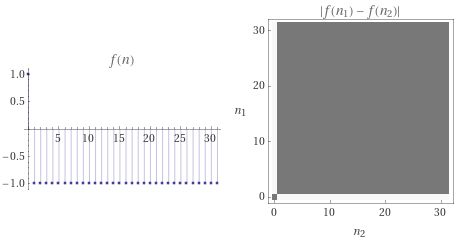
\includegraphics[scale=1.0]{wykresZad6a}
      \centering
      \caption{Wykres dla $c=-2$ i $x_{0}=1$}
    \end{figure}

    \begin{table}[H]
    \centering
    \begin{tabular}{|c | c |} 
     \hline
     x & Wartość \\ [0.5ex]
     \hline\hline
     $x_{0}$ & $2.0$ \\
     $x_{1}$ & $2.0$ \\
     $x_{2}$ & $2.0$ \\
     $x_{3}$ & $2.0$ \\
     $x_{4}$ & $2.0$  \\
     $x_{5}$ & $2.0$ \\
     ... & ... \\
     $x_{41}$ & $2.0$ \\
     \hline
    \end{tabular}
    \caption{Wyniki dla $c=-2$ i $x_{0}=2$}
    \label{Zad6b}
    \end{table}
    \begin{figure}[H]
      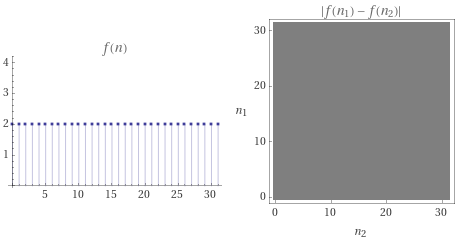
\includegraphics[scale=1.0]{wykresZad6b}
      \centering
      \caption{Wykres dla $c=-2$ i $x_{0}=2$}
    \end{figure}

    \begin{table}[H]
    \centering
    \begin{tabular}{|c | c |} 
     \hline
     x & Wartość \\ [0.5ex]
     \hline\hline
     $x_{0}$ & $1.99999999999999$ \\
     $x_{1}$ & $1.99999999999996$ \\
     $x_{2}$ & $1.9999999999998401$ \\
     $x_{3}$ & $1.9999999999993605$ \\
     $x_{4}$ & $1.999999999997442$  \\
     $x_{5}$ & $1.9999999999897682$ \\
     ... & ... \\
     $x_{41}$ & $-0.3289791230026702 $ \\
     \hline
    \end{tabular}
    \caption{Wyniki dla $c=-2$ i $x_{0}=1.99999999999999$}
    \label{Zad6c}
    \end{table}
    \begin{figure}[H]
      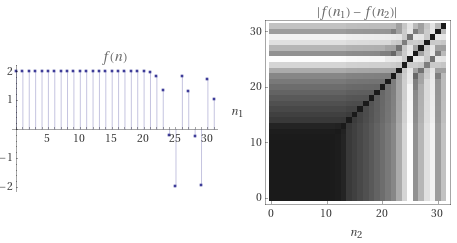
\includegraphics[scale=1.0]{wykresZad6c}
      \centering
      \caption{Wykres dla $c=-2$ i $x_{0}=1.99999999999999$}
    \end{figure}

    \begin{table}[H]
    \centering
    \begin{tabular}{|c | c |} 
     \hline
     x & Wartość \\ [0.5ex]
     \hline\hline
     $x_{0}$ & $1.0$ \\
     $x_{1}$ & $0.0$ \\
     $x_{2}$ & $-1.0$ \\
     $x_{3}$ & $0.0$ \\
     $x_{4}$ & $-1.0$  \\
     $x_{5}$ & $0.0$ \\
     ... & ... \\
     $x_{41}$ & $-1.0 $ \\
     \hline
    \end{tabular}
    \caption{Wyniki dla $c=-1$ i $x_{0}=1$}
    \label{Zad6d}
    \end{table}
    \begin{figure}[H]
      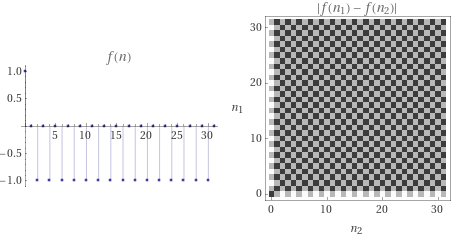
\includegraphics[scale=1.0]{wykresZad6d}
      \centering
      \caption{Wykres dla $c=-1$ i $x_{0}=1$}
    \end{figure}

    \begin{table}[H]
    \centering
    \begin{tabular}{|c | c |} 
     \hline
     x & Wartość \\ [0.5ex]
     \hline\hline
     $x_{0}$ & $-1.0$ \\
     $x_{1}$ & $0.0$ \\
     $x_{2}$ & $-1.0$ \\
     $x_{3}$ & $0.0$ \\
     $x_{4}$ & $-1.0$  \\
     $x_{5}$ & $0.0$ \\
     ... & ... \\
     $x_{41}$ & $-1.0 $ \\
     \hline
    \end{tabular}
    \caption{Wyniki dla $c=-1$ i $x_{0}=-1$}
    \label{Zad6e}
    \end{table}
    \begin{figure}[H]
      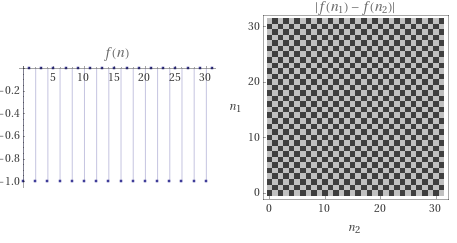
\includegraphics[scale=1.0]{wykresZad6e}
      \centering
      \caption{Wykres dla $c=-1$ i $x_{0}=-1$}
    \end{figure}

    \begin{table}[H]
    \centering
    \begin{tabular}{|c | c |} 
     \hline
     x & Wartość \\ [0.5ex]
     \hline\hline
     $x_{0}$ & $0.75$ \\
     $x_{1}$ & $-0.4375$ \\
     $x_{2}$ & $-0.80859375$ \\
     $x_{3}$ & $-0.3461761474609375$ \\
     $x_{4}$ & $-0.8801620749291033$  \\
     $x_{5}$ & $-0.2253147218564956$ \\
     ... & ... \\
     $x_{41}$ & $-1.0 $ \\
     \hline
    \end{tabular}
    \caption{Wyniki dla $c=-1$ i $x_{0}=0.75$}
    \label{Zad6f}
    \end{table}
    \begin{figure}[H]
      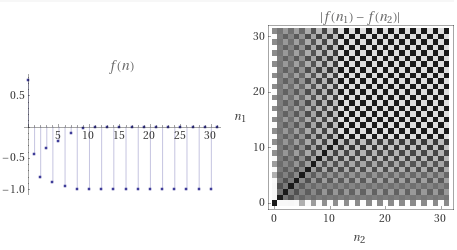
\includegraphics[scale=1.0]{wykresZad6f}
      \centering
      \caption{Wykres dla $c=-1$ i $x_{0}=0.75$}
    \end{figure}

    \begin{table}[H]
    \centering
    \begin{tabular}{|c | c |} 
     \hline
     x & Wartość \\ [0.5ex]
     \hline\hline
     $x_{0}$ & $0.25$ \\
     $x_{1}$ & $-0.9375$ \\
     $x_{2}$ & $-0.12109375$ \\
     $x_{3}$ & $-0.9853363037109375$ \\
     $x_{4}$ & $-0.029112368589267135$  \\
     $x_{5}$ & $-0.9991524699951226$ \\
     ... & ... \\
     $x_{41}$ & $0.0 $ \\
     \hline
    \end{tabular}
    \caption{Wyniki dla $c=-1$ i $x_{0}=0.25$}
    \label{Zad6g}
    \end{table}
    \begin{figure}[H]
      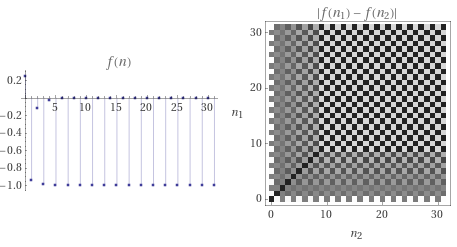
\includegraphics[scale=1.0]{wykresZad6g}
      \centering
      \caption{Wykres dla $c=-1$ i $x_{0}=0.25$}
    \end{figure}
    \textbf{Interpretacja: } Dla całkowitych wartości $x$ otrzymane wyniki zgadzają się z naszą intuicją, jednakże sytuacja nie jest tak dobra przy użyciu liczb zmiennoprzecinkowych. Ze względu na fakt, iż w ów funkcji rekurencyjnej jeden z elementów jest podnoszony do kwadratu liczba cyfr znaczących po przecinku podwaja się w każdym ruchu. Już na etapie 4 iteracji widzimy, że sprawia to nielada problem. Ów zachowanie uniemożliwia otrzymanie dokładnych wyników. \\
    Dodatkowo zauważamy, iż dla $x_{0}=0.25$ oraz $x_{0}=0.75$ zachowanie funkcji w pewnym momencie zaczyna być podobne jak dla $x_{0}=1$ i $x_{0}=2$, natomiast użycie $x_{0}=1.99999999999999$ skutkuje całkowita rozbieżnością względem oczekiwanych wyników (wynik zamiast "oddalać" się od zera to się do niego "przybliża")
  \section{Wnioski}
    Podobnie jak w zadaniu 5, niewielka niedokładność wartości $x_{0}$ przy odpowiednio dużej liczbie iteracji doprowadziła do nawarstwienie się błędu do takiego stopnia, iż $x_{0}=1.99999999999999$ już przy 40 iteracjach zaczyna dawać zupełnie inne wyniki niż $x_{0}=2$. Wiąże się to, z niedokładnością reprezentacji liczb i wpływu tego zjawiska na błędy w wykonywanych działaniach.



\end{document}